% Para facilitar a manutenção é sempre melhore criar um arquivo por capitulo, para exemplo isso não é necessário

%---------------------------------------------------------------------------------------
\chapter{Descrição da execução do experimento}

	Para a realização deste experimento, foram utilizados o programa Quartus 13.0 SP 1 e a placa \ac{fpga}
Cyclone II - EP2C20F484C7.

	\section{ETAPA 1 – Display de 7 segmentos}
		Para representar um número de 4 \textit{bits} na placa, utilizou-se 4 \textit{switch}, cada um
		representando um bit do número. Como um segmento do \textit{display} pode ser acendido
		em mais de um número,
		motou-se uma expressão lógica para cada segmento do \textit{display}.

		\begin{table}[h]
			\centering
			\caption{Tabela verdade utilizada para chegar na expressão de cada um dos segmentos.}
			\label{table:tabelaVerdade1}
			\begin{tabular}{c|c|c|c|c}
		%\hline
				\textbf{A (SW[4])} & \textbf{B (SW[3])} & \textbf{C (SW[2])} & \textbf{D (SW[1])} & \textbf{Saída em base decimal} \\
				\hline
				0 & 0 & 0 & 0 & 0\\
				0 & 0 & 0 & 1 & 1\\
				0 & 0 & 1 & 0 & 2\\
				0 & 0 & 1 & 1 & 3\\
				0 & 1 & 0 & 0 & 4\\
				0 & 1 & 0 & 1 & 5\\
				0 & 1 & 1 & 0 & 6\\
				0 & 1 & 1 & 1 & 7\\
				1 & 0 & 0 & 0 & 8\\
				1 & 0 & 0 & 1 & 9\\
			\end{tabular}
		\end{table}

		Para o segmento 0 montou-se a expressão
		$$\overline{A}.\overline{B}.\overline{C}.D+\overline{A}.B.\overline{C}.\overline{D}$$
		para o segmento 1 montou-se a expressão
		$$\overline{A}.B.\overline{C}.D+\overline{A}.B.C.\overline{D}$$
		para o segmento 2 montou-se a expressão
		$$\overline{A}.\overline{B}.C.\overline{D}$$
		para o segmento 3 montou-se a expressão
		$$\overline{A}.B.\overline{C}.\overline{D}+\overline{A}.\overline{B}.\overline{C}.D+\overline{A}.B.C.D$$
		para o segmento 4 montou-se a expressão
		$$\overline{A}.D+\overline{A}.B.\overline{C}+\overline{B}.\overline{C}.D$$
		para o segmento 5 montou-se a expressão
		$$\overline{A}.\overline{B}.D+\overline{A}.C.D+\overline{A}.\overline{B}.C$$
		para o segmento 6 montou-se a expressão
		$$\overline{A}.\overline{B}.\overline{C}+\overline{A}.B.C.D$$.

		Com tais expressões, montou-se um módulo em Verilog conforme \autoref{dec}.



		\begin{lstlisting}[frame=L, caption={Módulo de decodificação.},label=dec]  % Start your code-block

		module decodificacao ( A, B, C, D, h0, h1, h2, h3, h4, h5, h6);
			input A, B, C, D;
			output h0, h1, h2, h3, h4, h5, h6;

			assign h0 = (~A&~B&~C&D) | (~A&B&~C&~D);
			assign h1 = (~A&B&~C&D) | (~A&B&C&~D);
			assign h2 = ~A&~B&C&~D;
			assign h3 = (~A&B&~C&~D) | (~A&~B&~C&D) | (~A&B&C&D);
			assign h4 = (~A&D) | (~A&B&~C) | (~B&~C&D);
			assign h5 = (~A&~B&D) | (~A&C&D) | (~A&~B&C);
			assign h6 = (~A&~B&~C) | (~A&B&C&D);

		endmodule
		\end{lstlisting}

		Depois foram realizadas simulações e execução do circuito na placa \ac{fpga}.

	\section{ETAPA 2 – Meio-somador 1 bit}

		A operação aritmética mais simples é a soma de dois dígitos binários. Um circuito combinacional
		que implementa a adição de dois bits é chamado de meio-somador (half adder ou HAD).
		A \autoref{fig:meioSomador} ilustra um esquema de entradas e saída de um meio-somador.
		Um meio-somador de 1 bit deve respeitar a \autoref{table:tabelaMeioSomador}.

		\begin{figure}[H]
			\centering
			\caption{\label{fig:meioSomador}Ilustração de um meio somador.}
			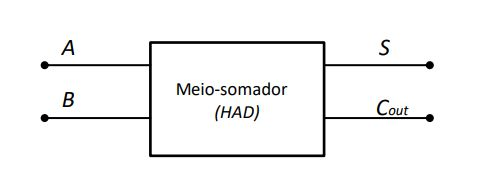
\includegraphics[width=1\textwidth]{img/meioSomador}
		\end{figure}

		\begin{table}[h]
			\centering
			\caption{Tabela verdade de um meio somador.}
			\label{table:tabelaMeioSomador}
			\begin{tabular}{c|c|c|c}
		%\hline
				\textbf{A} & \textbf{B} & \textbf{S (soma)} & \textbf{CarryOut} \\
				\hline
				0 & 0 & 0 & 0\\
				0 & 1 & 1 & 0\\
				1 & 0 & 1 & 0\\
				1 & 1 & 0 & 1\\
			\end{tabular}
		\end{table}

		O circuito deve guardar o \textit{CarryOut} ( o “vai um”) da soma, representando sua existência
		ou ausência através de um LED, ligando-o quando houver o carry, e mantendo-o desligado quando
		o carry não ocorrer.

		Então montou-se o módulo de meio-somador, conforme \autoref{meio-somador}.
		\begin{lstlisting}[frame=L, caption={Módulo do meio somador.},label=meio-somador]  % Start your code-block

		module meio_somador2 ( a, b, soma, cout);
    		input a, b;
    		output soma, cout;

	 		assign soma = a ^ b;
    		assign cout = a * b;

		endmodule
		\end{lstlisting}

	\section{ETAPA 3 – Meio-somador 4 bits}
		Foi montato o somador completo, ou seja,levando em consideração o "vai um",
		 depois fez-se os testes.
		Por fim, dividiu-se o resultado em dois display conforme o \autoref{projeto}.
		\begin{lstlisting}[frame=L, caption={Módulo do somador completo e suas dependências.},label=projeto]  % Start your code-block

		module meio_somador2 ( a, b, soma, cout);
    		input a, b;
    		output soma, cout;

	 		assign soma = a ^ b;
    		assign cout = a * b;

		endmodule

		module meio_somador3 ( a, b, c, soma, cout);
		    input a, b, c;
		    output soma, cout;

			wire carry_1, carry_2, soma_1;

		    meio_somador2 m1 ( a, b, soma_1, carry_1);
		    meio_somador2 m2 (soma_1, c, soma, carry_2);

			or o (cout, carry_1, carry_2);

		endmodule

		module somador_4_bits (a1, a2, b1, b2, c1, c2, d1, d2, soma1, soma2, soma3, soma4, cout);
			input a1, a2, b1, b2, c1, c2, d1, d2;
			output soma1, soma2, soma3, soma4, cout;

			wire carry_1, carry_2, carry_3;

			meio_somador2 s1 ( a1, a2, soma1, carry_1);
			meio_somador3 s2 ( b1, b2, carry_1, soma2, carry_2);
			meio_somador3 s3 ( c1, c2, carry_2, soma3, carry_3);
			meio_somador3 s4 ( d1, d2, carry_3, soma4, cout);

		endmodule

		module separa ( A, B, C, D, E, z0, z1, z2, z3, z4);
			input A, B, C, D, E;
			output z0, z1, z2, z3, z4;

			assign z0 = (~A&E) | (~B&~C&~D&E);
			assign z1 = (~A&~B&D) | (~A&B&C&~D) | (A&~B&~C&~D);
			assign z2 = (~A&~B&C) | (~A&C&D) | (A&~B&~C&~D);
			assign z3 = (~A&B&~C&~D) | (A&~B&~C&D&~E);
			assign z4 = (~A&B&D) | (~A&B&C) | (A&~B&~C&~D) | (A&~B&~C&~E);

		endmodule

		module decodificacao ( A, B, C, D, h0, h1, h2, h3, h4, h5, h6);
			input A, B, C, D;
			output h0, h1, h2, h3, h4, h5, h6;

			assign h0 = (~A&~B&~C&D) | (~A&B&~C&~D);
			assign h1 = (~A&B&~C&D) | (~A&B&C&~D);
			assign h2 = ~A&~B&C&~D;
			assign h3 = (~A&B&~C&~D) | (~A&~B&~C&D) | (~A&B&C&D);
			assign h4 = (~A&D) | (~A&B&~C) | (~B&~C&D);
			assign h5 = (~A&~B&D) | (~A&C&D) | (~A&~B&C);
			assign h6 = (~A&~B&~C) | (~A&B&C&D);

		endmodule

		module projeto (SW, HEX0, HEX1);
			input [7:0]SW;
			output [6:0] HEX0,HEX1;
			wire z0, z1, z2, z3, z4, z5, z6, z7;

			wire s1, s2, s3, s4, cout;

			somador_4_bits soma ( SW[0], SW[4], SW[1], SW[5], SW[2], SW[6], SW[3], SW[7], s1, s2, s3, s4, cout);
			separa s (cout, s4, s3, s2, s1, z0, z1, z2, z3, z4);

			assign z5 = 0;
			assign z6 = 0;
			assign z7 = 0;

			decodificacao dec1 ( z3, z2, z1, z0, HEX0[0], HEX0[1], HEX0[2], HEX0[3], HEX0[4], HEX0[5], HEX0[6]);
			decodificacao dec2 ( 0, 0, 0, z4, HEX1[0], HEX1[1], HEX1[2], HEX1[3], HEX1[4], HEX1[5], HEX1[6]);

		endmodule
		\end{lstlisting}




%Apresentar   o   detalhamento   da  execução  e   resultados   dos   passos   realizados
%durante   o   experimento,   incluindo   tabelas   verdade,   esquemáticos,   e   código
%(quando  houver).
%Especificar  componentes,  sistemas  e  instrumentos  utilizados.
%Usar listas, figuras e quadros, descrevê-los e discuti-los.



%---------------------------------------------------------------------------------------
